\section{Topographical Entropy Maximization}

Entropy maximization is any system parameter optimization which has the goal of maximizing system entropy. As an example, the entropy of a series of coin flips is maximized if the coin is "fair" with $p(h) = 1 - p(t) = 0.5$. For a graph, entropy is maximized where information centrality is minimized. As shown in Tables \ref{tab:unweighted_centrality} and \ref{tab:weighted_centrality}, changing the edge weights of Figure \ref{fig:simple_graph} results in different levels of entropy. In theory, a graph may have no identifiable most-central node. The most obvious form of such a graph would be one where only the "outer" links are present (a triangle for example). The end result would be equal information centrality for each node. Note, however, that the nodes of a triangle would have higher information centrality than those of a square etc. due to the greater optionality of the higher-sided shapes.

Entropy maximization can be readily applied to transportation planning. Take, for example, the road network diagrammed in Figure \ref{fig:divided_network}.

\begin{figure}[H]
	\centering
	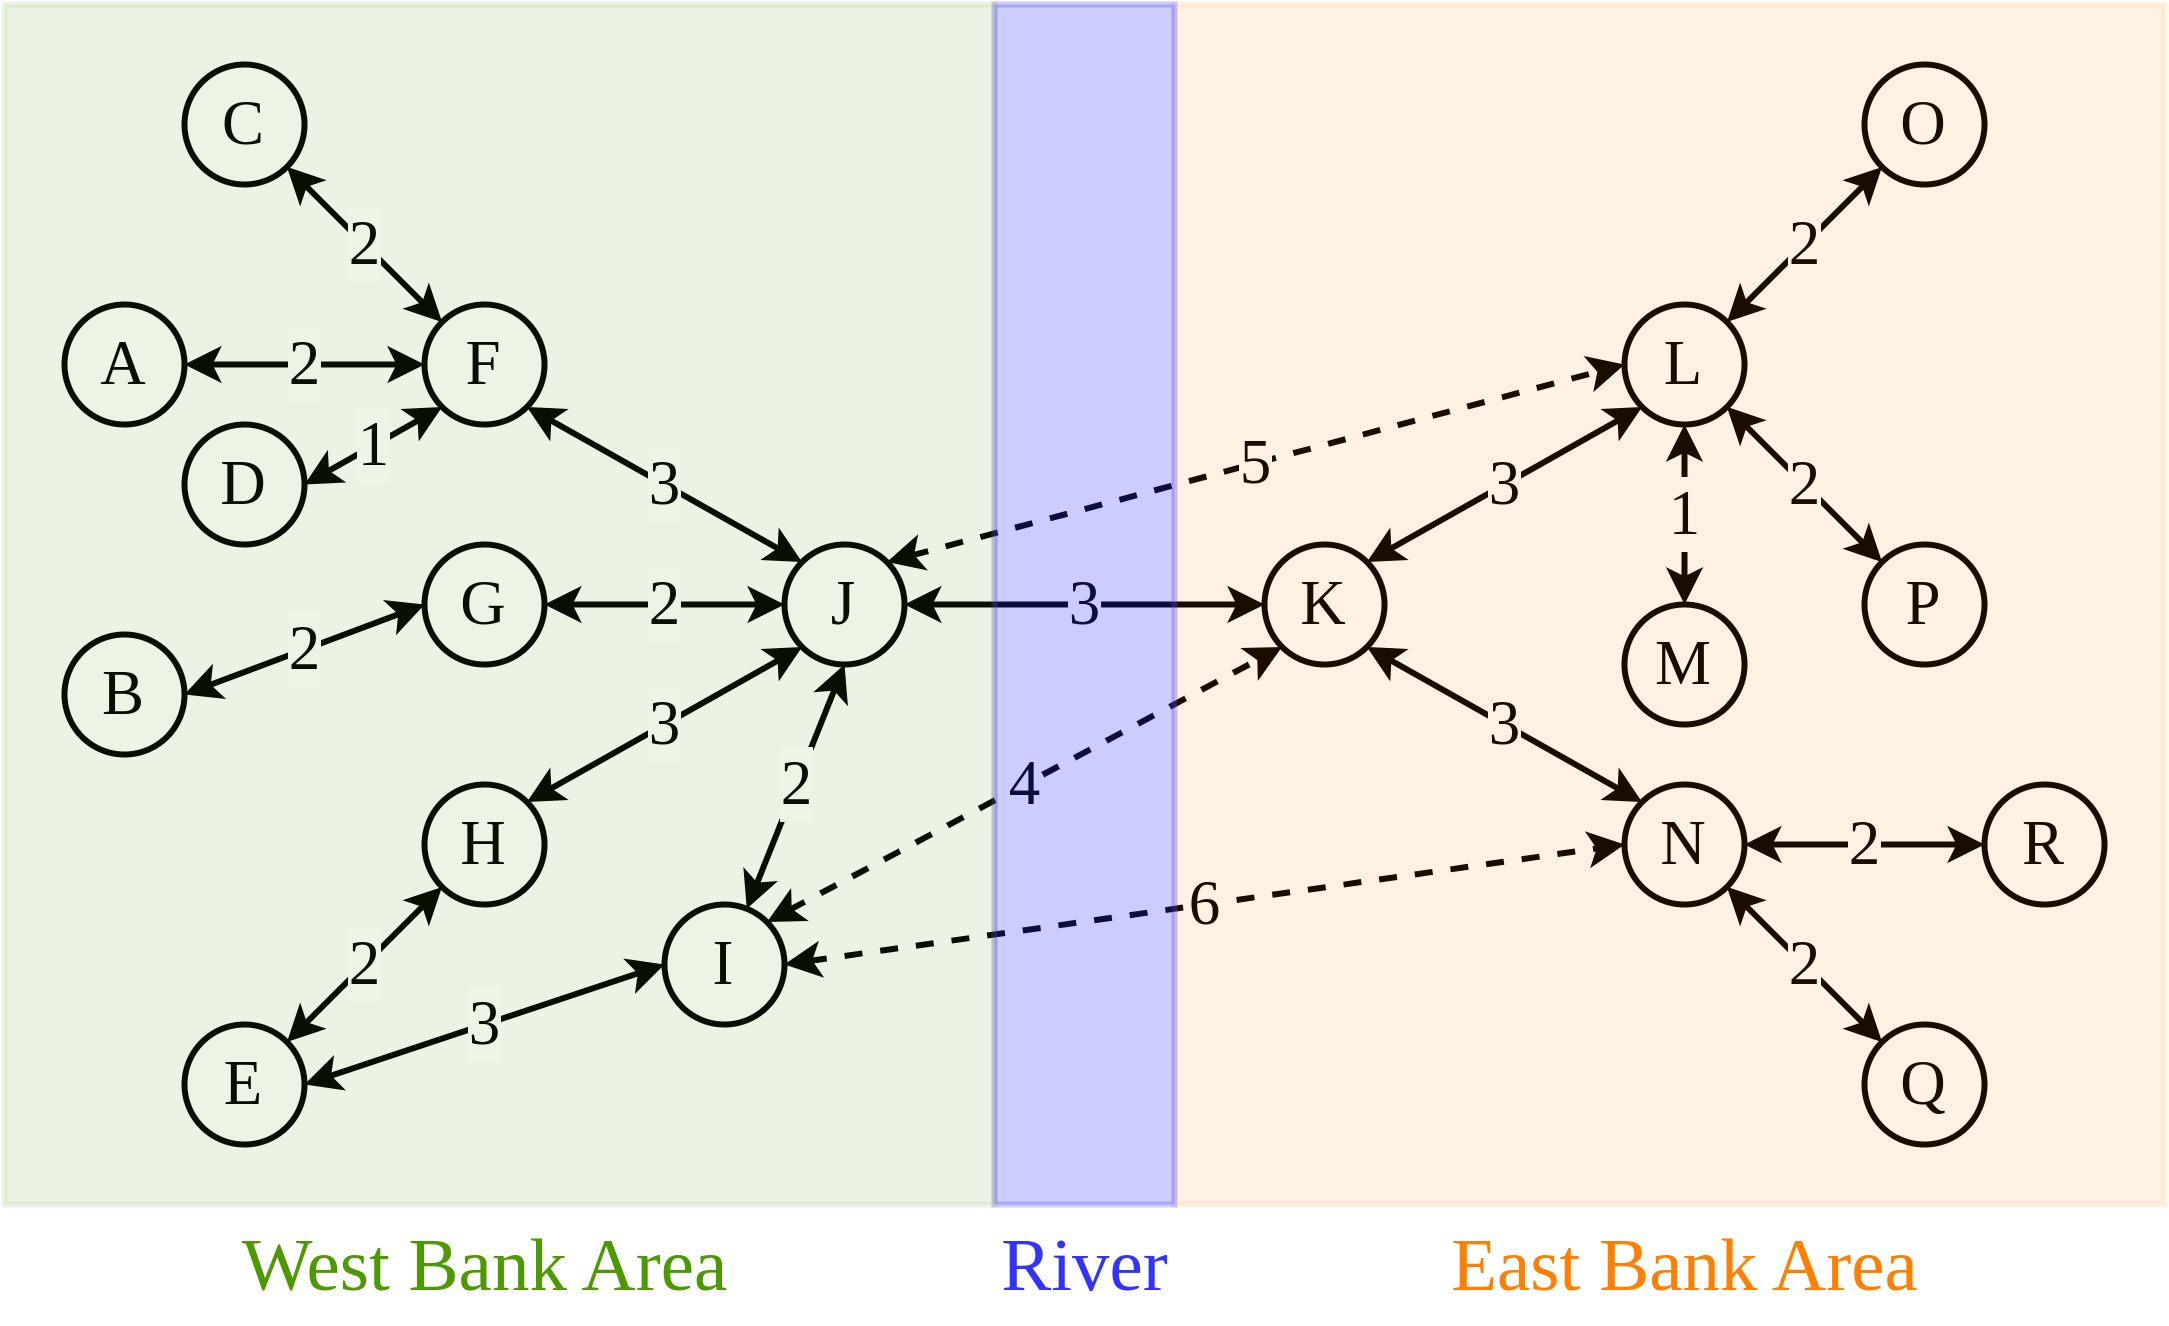
\includegraphics[width = .8\linewidth]{figs/divided_network.png}
	\caption{Example road network for city divided by a river. The solid links are present and dashed links are proposed additional links.}
	\label{fig:divided_network}
\end{figure}

The example city is, roughly, bifurcated by a river and the east and west bank areas are connected by a solitary bridge (J, K). It is evident that this bridge will feature in all shortest paths for O/D pairs on opposite sides of the river and is, thus both congested and a single point of failure for the network. Planners, thus, want to add at least one more bridge and have proposed the dashed links (I, N), (I, K), and (J, L). Information centrality for the network subject to the proposed additional bridges is listed in Table \ref{tab:bridge_information_centrality}.

\begin{table}[H]
	\centering
	\caption{Information centrality for example road network subject to bridge additions}
	\label{tab:bridge_information_centrality}
	\begin{tabular}{|C{.2\linewidth}|C{.2\linewidth}|C{.2\linewidth}|C{.2\linewidth}|C{.2\linewidth}|}
		\hline Node & Baseline & (I, N) & (I, K) & (J, L) \\
		\hline A & 0.0089 & 0.0083 & 0.0085 & 0.0088 \\
		\hline F & 0.0131 & 0.0127 & 0.0128 & 0.0137 \\
		\hline B & 0.0078 & 0.0072 & 0.0074 & 0.0076 \\
		\hline G & 0.0108 & 0.0102 & 0.0104 & 0.0109 \\
		\hline C & 0.0089 & 0.0083 & 0.0085 & 0.0088 \\
		\hline D & 0.0068 & 0.0062 & 0.0064 & 0.0065 \\
		\hline E & 0.0114 & 0.0124 & 0.0126 & 0.0117 \\
		\hline H & 0.0128 & 0.0129 & 0.0129 & 0.0133 \\
		\hline I & 0.0120 & 0.0146 & 0.0149 & 0.0123 \\
		\hline \textbf{J} & \textbf{0.0162} & \textbf{0.0162} & \textbf{0.0161} & \textbf{0.0177} \\
		\hline \textbf{K} & \textbf{0.0155} & \textbf{0.0153} & \textbf{0.0162} & \textbf{0.0157} \\
		\hline L & 0.0126 & 0.0122 & 0.0128 & 0.0164 \\
		\hline N & 0.0121 & 0.0147 & 0.0123 & 0.0119 \\
		\hline O & 0.0087 & 0.0081 & 0.0085 & 0.0099 \\
		\hline P & 0.0087 & 0.0081 & 0.0085 & 0.0099 \\
		\hline M & 0.0066 & 0.0061 & 0.0064 & 0.0071 \\
		\hline R & 0.0085 & 0.0092 & 0.0083 & 0.0081 \\
		\hline Q & 0.0085 & 0.0092 & 0.0083 & 0.0081 \\
		\hline \textbf{Sum} & \textbf{0.1899} & \textbf{0.1920} & \textbf{0.1917} & \textbf{0.1984} \\
		\hline
	\end{tabular}
\end{table}

Besides the obvious conclusion that adding a second bridge increases entropy, a few interesting observations can be made. First, that the (J, L) bridge increases overall entropy more than the (I, N) bridge both for the network in general and for node J in particular. Second that bridge (I, N) similarly outperforms bridge (I, K). Both can be explained by looking at the structure of the network in the east bank area. Because node I is fairly isolated compared to node J, extra bridges from node I provide less optionality than those from node J. The same can be said for nodes N and K.

Recall that entropy is the expectation of information for a set of events. Entropy is greater for a larger number of less likely events compared to a smaller number of more likely events. For example, the entropy of a "fair" coin flip is 1 bit while the entropy of a "fair" dice roll is 2.585 bits. The intuition of the results of the road network example is that bridge (J, L) was most effective in creating sub-optimal but plausible alternative routes thus reducing the load on (J, K). The maximal case of entropy in the network would occur if each node was incident to each other node by the same distance but this is not possible because the network nodes are at physical locations.